\section{Pose Estimation}


\subsection{Camera Matrix Estimation}

Pose estimation errors

Estimated camera matrix
\[ 
  P = \begin{bmatrix}
    1.19121690 \times 10^{-1} & 5.45061053 \times 10^{-1} & 1.90356266 \times 10^{-1} & -9.32574074 \times 10^{-2} \\
    -3.72738881 \times 10^{-1} & 1.96903454 \times 10^{-1} & -4.69365814 \times 10^{-1} & 4.95756458 \times 10^{-1} \\
    -2.82243252 \times 10^{-4} & -1.29896978 \times 10^{-4} & 6.42031422 \times 10^{-5} & 1.39340650 \times 10^{-3} \\
  \end{bmatrix}
\]

% P = array([[ 1.19121690e-01,  5.45061053e-01,  1.90356266e-01,
%         -9.32574074e-02],
%        [-3.72738881e-01,  1.96903454e-01, -4.69365814e-01,
%          4.95756458e-01],
%        [-2.82243252e-04, -1.29896978e-04,  6.42031422e-05,
%          1.39340650e-03]])

\begin{table}[H]
  \centering
  \begin{tabular}[2]{l | r |}
    \toprule
    \textbf{Metric} & \textbf{Value} \\
    \midrule
    Reprojection Error with clean 2D points & $1.510190084711698 \times 10^{-10}$ \\
    Pose Error with clean 2D points & $6.782416819715269 \times 10^{-12}$ \\
    Reprojection Error with noisy 2D points & $5.056479446706304$ \\
    Pose Error with noisy 2D points & $1.1255732262731768$ \\
    \bottomrule
  \end{tabular}
  \caption{Pose Estimation Errors (see Figure \ref{fig:raw-pose})}
\end{table}

\subsection{Intrinsic/Extrinsic Parameters Estimation}

% K = array([[-3.91311040e-01,  2.16322603e-02, -5.05036684e-01],
%        [ 0.00000000e+00, -5.79132614e-01, -3.84387155e-02],
%        [ 0.00000000e+00,  0.00000000e+00,  4.38131343e-04]])
% R = array([[-3.04416892e-01, -9.52538789e-01,  4.58882152e-04],
%        [ 9.52538627e-01, -3.04417134e-01, -6.10562418e-04],
%        [ 7.21275976e-04,  2.51237461e-04,  9.99999708e-01]])
% t = array([ 1.38022671, -4.14750766,  2.38863304])

\begin{align*}
  K &= \bmat{
    -3.91311040 \times 10^{-1} & 2.16322603 \times 10^{-2} & -5.05036684 \times 10^{-1} \\
    0.00000000 \times 10^{0} & -5.79132614 \times 10^{-1} & -3.84387155 \times 10^{-2} \\
    0.00000000 \times 10^{0} & 0.00000000 \times 10^{0} & 4.38131343 \times 10^{-4} \\
   } \\
  R &= \bmat{
    -3.04416892 \times 10^{-1} & -9.52538789 \times 10^{-1} & 4.58882152 \times 10^{-4} \\
    9.52538627 \times 10^{-1} & -3.04417134 \times 10^{-1} & -6.10562418 \times 10^{-4} \\
    7.21275976 \times 10^{-4} & 2.51237461 \times 10^{-4} & 9.99999708 \times 10^{-1} \\
  } \\
  t &= \bmat{
    1.38022671 // -4.14750766 // 2.38863304 \\
  }
\end{align*}

\begin{table}[H]
  \centering
  \begin{tabular}[2]{l | r |}
    \toprule
    \textbf{Metric} & \textbf{Value} \\
    \midrule
    Intrinsic Error with clean 2D points & $141.45256375245376$ \\
    Rotation Error with clean 2D points & $1.8653823929245028$ \\
    Translation Error with clean 2D points & $3.0626221861668257$ \\
    Intrinsic Error with noisy 2D points & $141.45251343470733$ \\
    Rotation Error with noisy 2D points & $1.8735506641560857$ \\
    Translation Error with noisy 2D points & $4.420673631875621$ \\
    \bottomrule
  \end{tabular}
  \caption{Intrinsics/Extrinsics Estimation Errors (see Figure \ref{fig:raw-intrinsics-error})}
\end{table}

\newpage
\subsection{CAD Alignment and Projection}

An aeroplane CAD model aligned onto an image
using calculated depth information.

% figure of the 3 images:
% - projected-points
% - warped cad
% - projected-cad
% use minipages to fit all 3 horizontally

\begin{figure}[H]
  \centering
  % minipage
  \begin{minipage}{\textwidth}
    \centering
    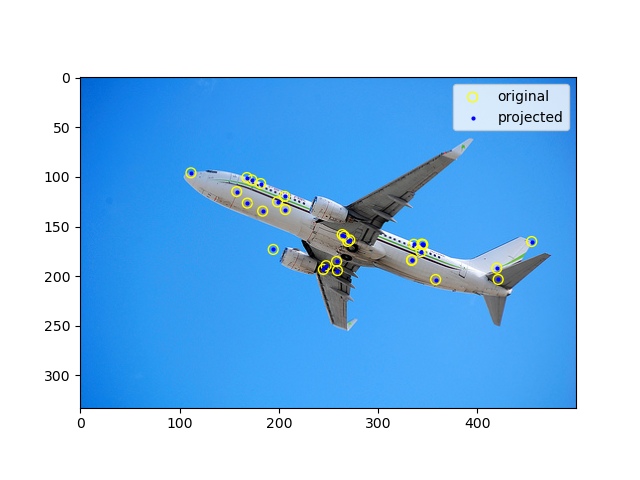
\includegraphics[width=\textwidth]{./figures/03-projected-points-2.png}
    \caption*{Points Projected onto Image}
  \end{minipage}
\end{figure}

\begin{figure}[H]
  \centering
  % minipage
  \begin{minipage}{.49\textwidth}
    \centering
    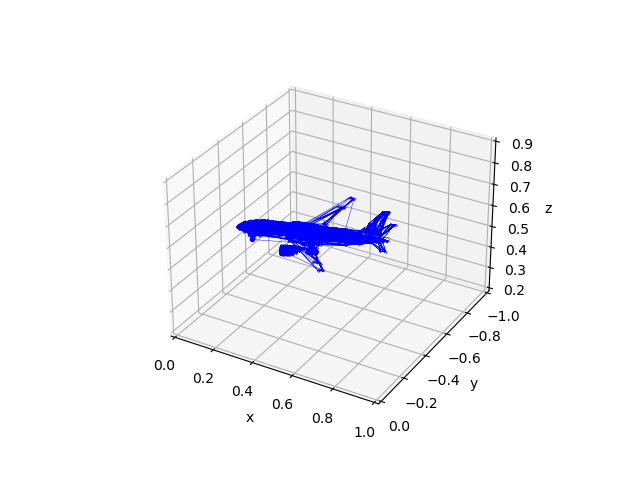
\includegraphics[width=\textwidth]{./figures/03-warped-cad-4.png}
    \caption*{Warped CAD (no rotation)}
  \end{minipage}
  \hfill
  % minipage
  \begin{minipage}{.49\textwidth}
    \centering
    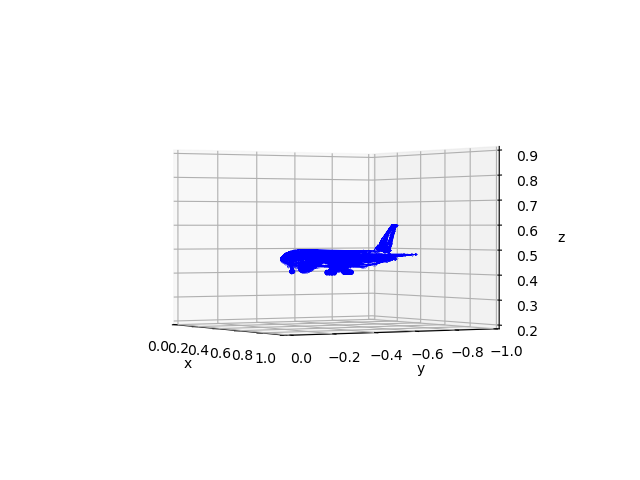
\includegraphics[width=\textwidth]{./figures/03-warped-cad-2.png}
    \caption*{Perspective $2$}
  \end{minipage}
\end{figure}
\begin{figure}
  \centering
  % minipage
  \begin{minipage}{.49\textwidth}
    \centering
    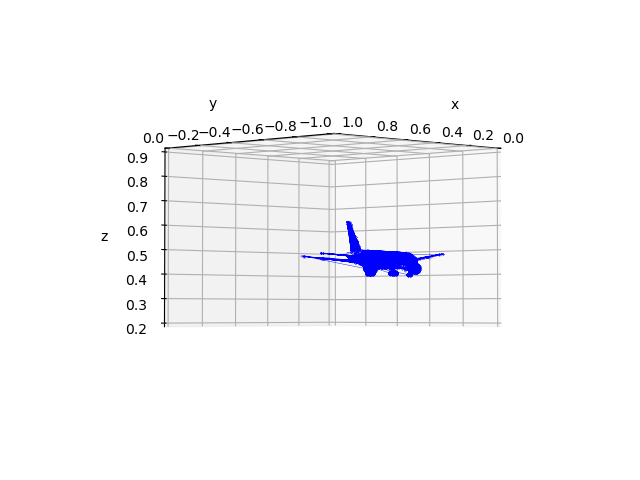
\includegraphics[width=\textwidth]{./figures/03-warped-cad-3.png}
    \caption*{Perspective $3$}
  \end{minipage}
  \hfill
  % minipage
  \begin{minipage}{.49\textwidth}
    \centering
    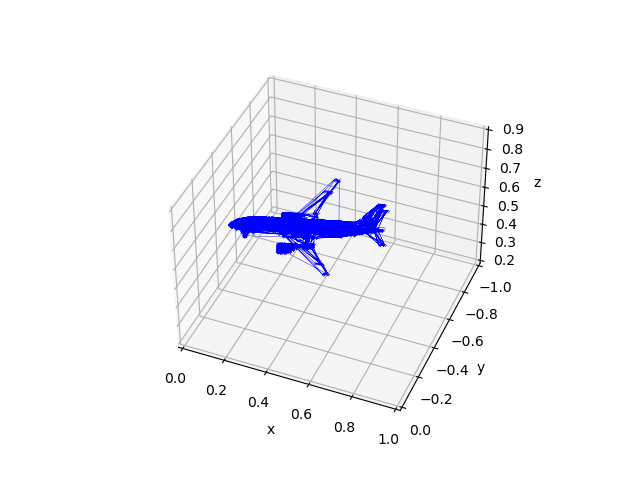
\includegraphics[width=\textwidth]{./figures/03-warped-cad-1.png}
    \caption*{Perspective $4$}
  \end{minipage}
\end{figure}

\begin{figure}[H]
  \centering
  % minipage
  \begin{minipage}{.8\textwidth}
    \centering
    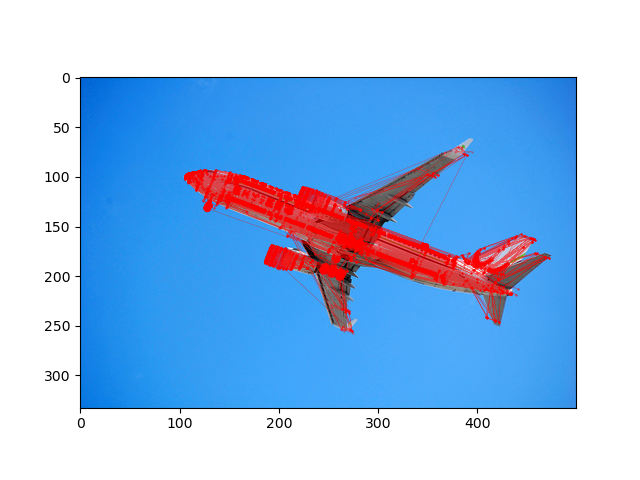
\includegraphics[width=\textwidth]{./figures/03-warped-cad.png}
    \caption*{Warped CAD}
  \end{minipage}
\end{figure}
